\definecolor{olivegreen}{RGB}{91,130,0}
\definecolor{crimsonred}{RGB}{192,0,0}
\definecolor{deepblue}{RGB}{0,70,175}
\definecolor{darkorange}{RGB}{200,90,0}


\begin{figure}[t]
\centering
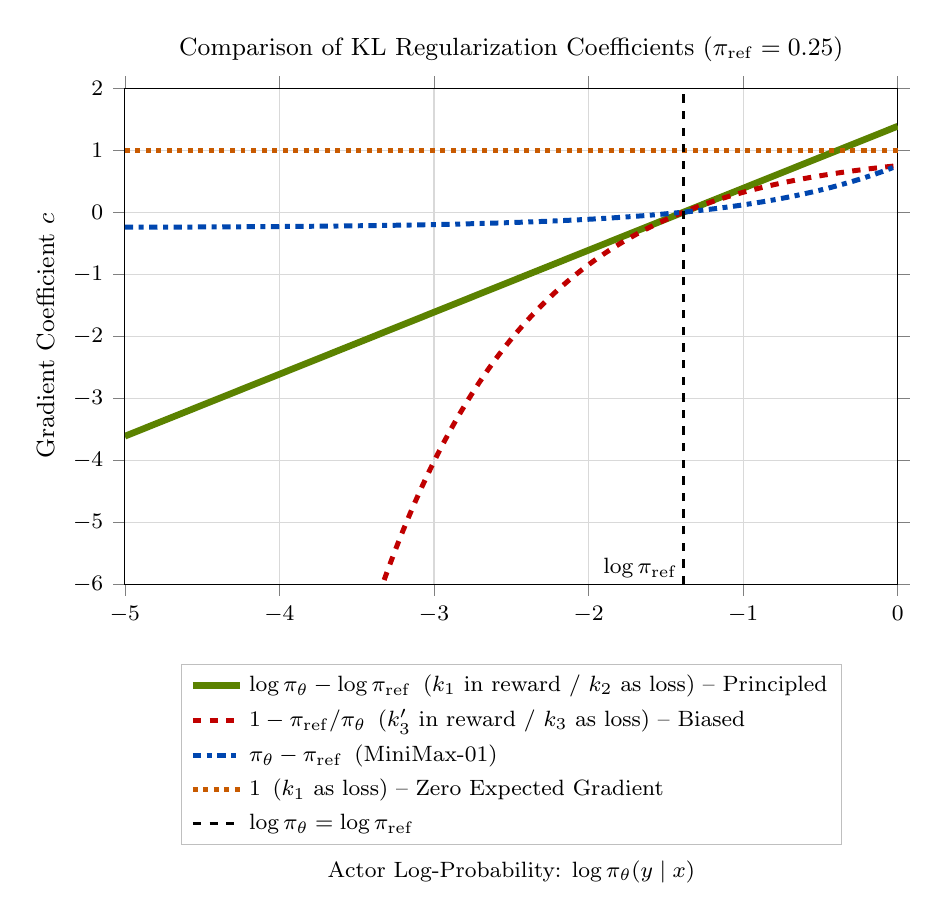
\begin{tikzpicture}
\pgfplotsset{
    clip marker paths=true,
}
\begin{axis}[
    name=mainplot,
    width=0.94\linewidth,
    height=0.65\linewidth,
    xmin=-5, xmax=0,
    ymin=-6, ymax=2,
    enlarge x limits=false,
    xlabel={},
    ylabel={Gradient Coefficient $c$},
    title={Comparison of KL Regularization Coefficients ($\pi_{\mathrm{ref}} = 0.25$)},
    title style={font=\small},
    ylabel style={font=\small},
    label style={font=\small},
    tick label style={font=\footnotesize},
    legend style={
        name=kl legend,
        at={(0.5,-0.16)},
        anchor=north,
        legend columns=1,
        font=\footnotesize,
        draw=gray!50,
        fill=white,
        legend cell align=left,
        row sep=1pt,
    },
    grid=both,
    minor grid style={gray!15},
    major grid style={gray!30},
    tick align=outside,
    xtick={-5,-4,-3,-2,-1,0},
    ytick={-6,-5,-4,-3,-2,-1,0,1,2},
    clip=true,
]

%% log pi_theta - log pi_ref  (Principled)
\addplot[
    color=olivegreen, line width=2.4pt, solid,
    domain=-5:0, samples=300,
]{x - ln(0.25)};
\addlegendentry{$\log \pi_\theta - \log \pi_{\mathrm{ref}}$\enspace
    ($k_1$ in reward / $k_2$ as loss) -- Principled}

%% 1 - pi_ref/pi_theta  (Biased Approximation)
\addplot[
    color=crimsonred, line width=1.8pt, dashed,
    domain=-5:0, samples=300,
]{1 - 0.25*exp(-x)};
\addlegendentry{$1 - \pi_{\mathrm{ref}}/\pi_\theta$\enspace
    ($k_3'$ in reward / $k_3$ as loss) -- Biased}

%% pi_theta - pi_ref  (MiniMax-01)
\addplot[
    color=deepblue, line width=1.8pt, dash dot,
    domain=-5:0, samples=300,
]{exp(x) - 0.25};
\addlegendentry{$\pi_\theta - \pi_{\mathrm{ref}}$\enspace (MiniMax-01)}

%% constant 1  (Zero Expected Gradient)
\addplot[
    color=darkorange, line width=1.8pt, dotted,
    domain=-5:0,
]{1};
\addlegendentry{$1$\enspace ($k_1$ as loss) -- Zero Expected Gradient}

%% Vertical dashed line at log(0.25)
\draw[black, line width=1.2pt, dashed] (axis cs:-1.3863, -6) -- (axis cs:-1.3863, 2);
\addlegendimage{black, dashed, line width=1.2pt}
\addlegendentry{$\log \pi_\theta = \log \pi_{\mathrm{ref}}$}

\node[anchor=south east, font=\footnotesize, inner sep=2pt, overlay]
    at (axis cs:-1.3863, -6) {$\log \pi_{\mathrm{ref}}$};

\end{axis}

%% xlabel
\node[anchor=north, font=\footnotesize, below=2pt] at (kl legend.south)
    {Actor Log-Probability: $\log \pi_\theta(y \mid x)$};

\end{tikzpicture}
\caption{Comparison of the gradient coefficient~$c$
that each KL implementation induces on the score function
$\nabla_\theta\log\pi_\theta$
(plotted against $\log \pi_\theta(y|x)$; $\pi_{\mathrm{ref}} = 0.25$).
The principled RKL implementations
($\boldsymbol{k_1}$~\textbf{in reward} and
$\boldsymbol{k_2}$~\textbf{as loss}) yield $c = k_1$.
The GRPO-style $\boldsymbol{k_3}$~\textbf{as loss} produces
$c = 1 - \delta$ ($\delta = \pi_{\mathrm{ref}}/\pi_\theta$),
a first-order approximation with mismatched tails.
The direct $\boldsymbol{k_1}$~\textbf{as loss} yields
a constant $c = 1$, producing zero-mean noise.}
\label{fig:kl-coeff}
\end{figure}
